% !TEX program = xelatex
\makeatletter\let\@expl@@@mark@update@singlecol@structures@@\relax\makeatother
\documentclass[11pt,a4paper]{article}

% -------------------- កញ្ចប់ពុម្ពអក្សរ និងភាសា --------------------
\usepackage{fontspec}
\usepackage{amsmath,amssymb}
\usepackage{unicode-math}
\usepackage{pifont}

% -------------------- ការកំណត់ទំព័រ (២ ទំព័រ A4 ស-ខ្មៅ ពេញសមត្ថភាព) --------------------
\usepackage[
  a4paper,
  left=1.10cm,
  right=1.10cm,
  top=1.05cm,
  bottom=1.15cm,
  footskip=0.55cm
]{geometry}

\usepackage{fancyhdr}
\usepackage{array}
\usepackage{colortbl}
\usepackage[table]{xcolor}
\usepackage{tikz}
\usetikzlibrary{calc,angles,quotes,arrows.meta}
\usepackage[most]{tcolorbox}

% -------------------- ពុម្ពអក្សរ (Cross-Platform \NGSFindFonts) --------------------
\newcommand{\NGSFindFonts}{%
  \IfFileExists{C:/Windows/Fonts/cambria.ttc}{%
    \def\NGSSysPath{C:/Windows/Fonts/}%
    \def\NGSUserPath{C:/Users/KIT/AppData/Local/Microsoft/Windows/Fonts/}%
  }{%
    \IfFileExists{./fonts/KhmerOSsiemreap.ttf}{\def\NGSSysPath{./fonts/}\def\NGSUserPath{./fonts/}}{%
    \IfFileExists{../fonts/KhmerOSsiemreap.ttf}{\def\NGSSysPath{../fonts/}\def\NGSUserPath{../fonts/}}{%
    \IfFileExists{../../fonts/KhmerOSsiemreap.ttf}{\def\NGSSysPath{../../fonts/}\def\NGSUserPath{../../fonts/}}{%
    \IfFileExists{../../../fonts/KhmerOSsiemreap.ttf}{\def\NGSSysPath{../../../fonts/}\def\NGSUserPath{../../../fonts/}}{%
    \IfFileExists{../../../../fonts/KhmerOSsiemreap.ttf}{\def\NGSSysPath{../../../../fonts/}\def\NGSUserPath{../../../../fonts/}}{%
    \IfFileExists{../../../../../fonts/KhmerOSsiemreap.ttf}{\def\NGSSysPath{../../../../../fonts/}\def\NGSUserPath{../../../../../fonts/}}{%
    \IfFileExists{../../../../../../fonts/KhmerOSsiemreap.ttf}{\def\NGSSysPath{../../../../../../fonts/}\def\NGSUserPath{../../../../../../fonts/}}{%
      \def\NGSSysPath{../../../../../../../fonts/}\def\NGSUserPath{../../../../../../../fonts/}%
    }}}}}}}%
  }%
}
\NGSFindFonts

\setmathfont[Path={\NGSSysPath}, FontIndex=1, Scale=1.02]{cambria.ttc}
\defaultfontfeatures{Ligatures=TeX}

\setmainfont[
  Path={\NGSUserPath}, Extension=.ttf, Script=Khmer,
  BoldFont={KhmerOSsiemreap}, BoldFeatures={FakeBold=1.8},
  ItalicFont={KhmerOSsiemreap}, ItalicFeatures={FakeSlant=0.22},
  BoldItalicFont={KhmerOSsiemreap}, BoldItalicFeatures={FakeBold=1.8, FakeSlant=0.22}
]{KhmerOSsiemreap}

\newfontfamily\muol[Path={\NGSUserPath}, Extension=.ttf, Script=Khmer]{KhmerOSmuollight}
\newfontfamily\LatinFont[Path={\NGSSysPath}, Extension=.ttf, BoldFont={timesbd}, ItalicFont={timesi}, BoldItalicFont={timesbi}]{times}

\XeTeXlinebreaklocale "km"
\XeTeXlinebreakskip = 0pt plus 1pt minus 0.1pt

\definecolor{ink}{HTML}{000000}
\definecolor{panelgray}{HTML}{F2F2F2}
\definecolor{headband}{HTML}{E4E4E4}

\newcommand{\en}[1]{{\LatinFont #1}}
\newcommand{\enbf}[1]{{\LatinFont\textbf{#1}}}
\newcommand{\unit}[1]{\,\text{\en{#1}}}
\newcommand{\cnum}[1]{{\fontsize{10pt}{11pt}\selectfont\ding{\numexpr181+#1\relax}}\hspace{0.15em}}
\newcommand{\blank}[1]{\underline{\hspace{#1}}}
\newcommand{\chkbox}{\tikz[baseline=-0.3ex]\draw[black,line width=0.7pt] (0,0) rectangle (0.31,0.31);}
\newcommand{\numbox}{\tikz[baseline=-0.35ex]\draw[black,line width=0.85pt] (0,0) rectangle (0.42,0.42);}

\newcommand{\secbox}[2]{%
  \vspace{4pt}%
  \noindent\begin{tcolorbox}[
    enhanced, sharp corners, boxrule=0.85pt, colframe=black, colback=headband,
    left=6pt, right=6pt, top=3pt, bottom=3pt, boxsep=1pt
  ]
    {\muol\fontsize{9.6pt}{13.5pt}\selectfont #1}\hfill{\fontsize{8.8pt}{12pt}\selectfont\textbf{#2}}
  \end{tcolorbox}%
  \vspace{2pt}%
}

\newcolumntype{L}[1]{>{\raggedright\arraybackslash}p{#1}}
\newcolumntype{C}[1]{>{\centering\arraybackslash}p{#1}}

\pagestyle{fancy}
\fancyhf{}
\renewcommand{\headrulewidth}{0pt}
\renewcommand{\footrulewidth}{0.4pt}
\fancyfoot[L]{\fontsize{8.5pt}{11pt}\selectfont អនុវិទ្យាល័យព្រះក្រសាំង \en{|} គណិតវិទ្យា ថ្នាក់ទី៧ \en{---} មេរៀនទី២ (១.១ ភាពចែកដាច់នឹង ២, ៥ និង ៣, ៩) \en{|} គ្រូ៖ ហុក ប៊ុនថែន}
\fancyfoot[R]{\fontsize{8.5pt}{11pt}\selectfont ទំព័រ \en{\thepage\ / 2}}

\setlength{\parindent}{0pt}
\setlength{\parskip}{0pt}
\setlength{\tabcolsep}{4pt}

\begin{document}
\fontsize{9.4pt}{13.9pt}\selectfont

% ============================================================================
% ទំព័រទី ១ ៖ ក្បាលសន្លឹកកិច្ចការ + ផ្នែក ក (E2 ពិសោធន៍ 2, 5 និង 3, 9) + ផ្នែក ខ (E3 សំយោគ & Warrant Bank)
% ============================================================================
\begin{tcolorbox}[
  enhanced, sharp corners, colback=white, colframe=black, boxrule=1.0pt,
  left=6pt, right=6pt, top=4pt, bottom=4pt, boxsep=1pt
]
  \begin{minipage}[c]{13.1cm}
    {\muol\fontsize{9.8pt}{14.2pt}\selectfont សន្លឹកកិច្ចការសិស្ស ២.១ ៖ ភាពចែកដាច់នៃចំនួនគត់នឹង \enbf{2, 5} និង \enbf{3, 9}}\\[3pt]
    ឈ្មោះសិស្ស៖ \blank{4.2cm} \quad ក្រុមទី៖ \blank{1.2cm} \quad ថ្នាក់ទី៧៖ \blank{1.2cm}\\[2pt]
    \textbf{បេសកកម្មឃ្លាំងសៀវភៅ \en{E1}៖} ដារ៉ាថា \textit{«$23$ ចុងលេខ $3$ ដាច់នឹង $3$ ឯ $207$ ចុងលេខ $7$ មិនដាច់នឹង $3, 9$»}៖ \chkbox\ ត្រូវ ឬ \chkbox\ ខុស? ហេតុអ្វី? \blank{2.0cm}
  \end{minipage}\hfill%
  \begin{minipage}[c]{4.75cm}
    \centering
    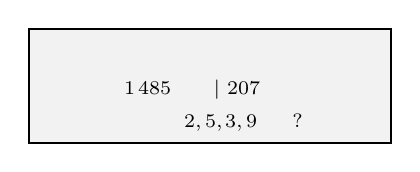
\begin{tikzpicture}[x=1cm, y=1cm, every node/.style={font=\scriptsize, text=black}]
      \draw[black, line width=0.8pt, fill=panelgray] (0,0) rectangle (4.60,1.45);
      \node at (2.30,1.12) {\textbf{ប្រអប់សៀវភៅឃ្លាំង៖}};
      \node at (2.30,0.68) {$1\,485$ ក្បាល \en{|} $207$ ក្បាល};
      \node at (2.30,0.26) {តើរៀបជាបាច់ $2, 5, 3, 9$ បានទេ?};
    \end{tikzpicture}
  \end{minipage}
\end{tcolorbox}

% -------------------- ផ្នែក ក (E2 Explore - 2 Stations: ÷2,÷5 and ÷3,÷9) --------------------
\secbox{ផ្នែក ក \enbf{(E2 Explore)} ៖ ពិសោធន៍ស្វែងរកក្បួនចែកដាច់នឹង \enbf{2, 5} និង \enbf{3, 9} (ទំ.១៥--១៦)}{១១ នាទី \en{---} គិតជាដៃគូ}

\textbf{ស្ថានីយទី១ (៥ នាទី)៖ ពិសោធន៍បំបែកដប់--រាយ ដើម្បីរកក្បួនចែកដាច់នឹង $2$ និង $5$ (សៀវភៅគោល ទំ.១៥)}\\[2pt]
{\renewcommand{\arraystretch}{1.44}
\fontsize{8.5pt}{12.2pt}\selectfont
\begin{tabular}{|C{1.35cm}|C{3.15cm}|C{2.05cm}|C{2.25cm}|C{2.25cm}|L{5.80cm}|}
  \hline
  \cellcolor{panelgray}\textbf{ចំនួន} & \cellcolor{panelgray}\textbf{បំបែកជាដប់ $+$ រាយ} & \cellcolor{panelgray}\textbf{លេខរាយចុង} & \cellcolor{panelgray}\textbf{ផលចែកនឹង $2$} & \cellcolor{panelgray}\textbf{ផលចែកនឹង $5$} & \cellcolor{panelgray}\textbf{សង្កេត (ដាច់នឹង $2$? នឹង $5$?)} \\ \hline
  $42$ & $4\times 10 + 2$ & $2$ & $21$ (សល់ $0$) & សល់ $2$ & \chkbox\ ដាច់នឹង $2$ \quad \chkbox\ ដាច់នឹង $5$ \\ \hline
  $43$ & $4\times 10 + 3$ & $3$ & សល់ $1$ & សល់ $3$ & មិនដាច់ទាំងពីរ (ព្រោះរាយ $3$!) \\ \hline
  $95$ & $9\times 10 + \blank{0.7cm}$ & \blank{0.8cm} & សល់ $1$ & \blank{1.4cm} & \chkbox\ ដាច់នឹង $2$ \quad \chkbox\ ដាច់នឹង $5$ \\ \hline
  $210$ & $\blank{0.7cm}\times 10 + \blank{0.7cm}$ & \blank{0.8cm} & \blank{1.4cm} & \blank{1.4cm} & \chkbox\ ដាច់នឹង $2$ \quad \chkbox\ ដាច់នឹង $5$ \\ \hline
  $525$ & $52\times 10 + \blank{0.7cm}$ & \blank{0.8cm} & សល់ $1$ & \blank{1.4cm} & \chkbox\ ដាច់នឹង $2$ \quad \chkbox\ ដាច់នឹង $5$ \\ \hline
\end{tabular}}

\vspace{5pt}
$\bullet$ \textbf{សន្និដ្ឋានស្ថានីយទី១៖} ព្រោះ $10 = 2 \times 5$ ចែកដាច់នឹង $2$ និង $5$ ជានិច្ច ដូច្នេះ៖ (ក) ដាច់នឹង $2$ កាលណាលេខរាយខាងចុងគឺ \blank{3.2cm} និង (ខ) ដាច់នឹង $5$ កាលណាលេខរាយខាងចុងគឺ \blank{1.9cm} ។

\vspace{6pt}
\textbf{ស្ថានីយទី២ (៦ នាទី)៖ ពិសោធន៍ «កាក់សំណល់ពីបាច់ $10$ និង $100$» រកក្បួនចែកដាច់នឹង $3$ និង $9$ (ទំ.១៦)}\\[3pt]
\begin{minipage}[t]{7.3cm}
  \vspace{0pt}
  \begin{tcolorbox}[
    enhanced, sharp corners, colback=panelgray, colframe=black,
    boxrule=0.8pt, boxsep=1.5pt, top=4pt, bottom=4pt, left=4pt, right=4pt
  ]
    \centering
    {\fontsize{8.2pt}{11.0pt}\selectfont\textbf{ហេតុអ្វីត្រូវបូកគ្រប់ខ្ទង់លេខ? ($216$ ចែកនឹង $3, 9$)}}\\[4pt]
    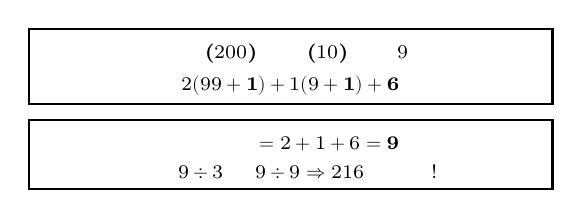
\begin{tikzpicture}[x=1cm, y=1cm, every node/.style={font=\scriptsize, text=black}]
      \draw[black, line width=0.8pt, fill=white] (0,1.12) rectangle (6.65,2.08);
      \node at (3.325,1.76) {\textbf{ខ្ទង់រយ ($200$) និងដប់ ($10$) ចែកនឹង $9$ ៖}};
      \node at (3.325,1.36) {$2(99+\mathbf{1}) + 1(9+\mathbf{1}) + \mathbf{6}$};

      \draw[black, line width=0.8pt, fill=white] (0,0.05) rectangle (6.65,0.92);
      \node at (3.325,0.62) {\textbf{កាក់សំណល់សរុប} $= 2 + 1 + 6 = \mathbf{9}$};
      \node at (3.325,0.26) {ព្រោះ $9 \div 3$ និង $9 \div 9 \Rightarrow 216$ ដាច់ទាំងពីរ!};
    \end{tikzpicture}\\[4pt]
    {\fontsize{8.0pt}{11.4pt}\selectfont ផ្ទៀងលេខដារ៉ា៖ $23 \div 3 = 7$ សល់ $\blank{0.6cm}$ (ផលបូក $2+3=\blank{0.6cm}$)}
  \end{tcolorbox}
\end{minipage}\hfill%
\begin{minipage}[t]{11.3cm}
  \vspace{0pt}
  {\renewcommand{\arraystretch}{1.42}
  \fontsize{8.3pt}{11.8pt}\selectfont
  \begin{tabular}{|C{1.25cm}|C{2.90cm}|C{1.35cm}|C{1.95cm}|C{1.95cm}|}
    \hline
    \cellcolor{panelgray}\textbf{ចំនួន} & \cellcolor{panelgray}\textbf{ផលបូកខ្ទង់លេខ} & \cellcolor{panelgray}\textbf{សរុប} & \cellcolor{panelgray}\textbf{ដាច់នឹង $3$?} & \cellcolor{panelgray}\textbf{ដាច់នឹង $9$?} \\ \hline
    $195$ & $1 + 9 + 5$ & $15$ & \chkbox\ បាទ \chkbox\ ទេ & \chkbox\ បាទ \chkbox\ ទេ \\ \hline
    $927$ & $9 + 2 + 7$ & \blank{0.9cm} & \chkbox\ បាទ \chkbox\ ទេ & \chkbox\ បាទ \chkbox\ ទេ \\ \hline
    $1\,005$ & \blank{2.2cm} & \blank{0.9cm} & \chkbox\ បាទ \chkbox\ ទេ & \chkbox\ បាទ \chkbox\ ទេ \\ \hline
    $828$ & \blank{2.2cm} & \blank{0.9cm} & \chkbox\ បាទ \chkbox\ ទេ & \chkbox\ បាទ \chkbox\ ទេ \\ \hline
    $123$ & $1 + 2 + 3$ & \blank{0.9cm} & \chkbox\ បាទ \chkbox\ ទេ & \chkbox\ បាទ \chkbox\ ទេ \\ \hline
  \end{tabular}}
\end{minipage}

\vspace{6pt}
% -------------------- ផ្នែក ខ (E3 Explain - Synthesis & Warrant Bank) --------------------
\secbox{ផ្នែក ខ \enbf{(E3 Explain)} ៖ សំយោគក្បួនទាំង ៤ និងធនាគារហេតុផល \enbf{(Warrant Bank)}}{៦ នាទី \en{---} បំពេញប្រអប់សំយោគ}

\begin{minipage}[t]{9.7cm}
  \vspace{2pt}\raggedright
  $\bullet$ \textbf{ក្រុមទី១ (មើលខ្ទង់ចុង — $2, 5$)៖} បើចំនួនមួយចែកដាច់នឹង $2$ \textbf{ផង} និង $5$ \textbf{ផង} នោះលេខខ្ទង់រាយខាងចុងត្រូវតែជាលេខ \blank{1.1cm} ជានិច្ច ។\\[5pt]
  $\bullet$ \textbf{ក្រុមទី២ (បូកគ្រប់ខ្ទង់ — $3, 9$)៖} ចែកដាច់នឹង $3$ កាលណា \blank{2.7cm} ចែកដាច់នឹង $3$; ចែកដាច់នឹង $9$ កាលណាផលបូកខ្ទង់ចែកដាច់នឹង \blank{0.9cm} ។\\[5pt]
  $\bullet$ \textbf{ទំនាក់ទំនង $9$ និង $3$៖} គ្រប់ចំនួនចែកដាច់នឹង $9$ ច្បាស់ជាចែកដាច់នឹង \blank{0.8cm} ជានិច្ច (តែច្រាសមកវិញមិនប្រាកដទេ ដូចជាលេខ $123$) ។
\end{minipage}\hfill%
\begin{minipage}[t]{8.9cm}
  \vspace{0pt}
  \begin{tcolorbox}[
    enhanced, sharp corners, colback=panelgray, colframe=black,
    boxrule=0.85pt, boxsep=2pt, top=4.5pt, bottom=4.5pt, left=5pt, right=5pt
  ]
    {\muol\fontsize{8.8pt}{12.5pt}\selectfont ធនាគារហេតុផល \enbf{(Warrant Bank)} សម្រាប់យោង៖}\\[3pt]
    {\fontsize{8.5pt}{13.4pt}\selectfont
    \cnum{1} \textbf{ដាច់នឹង $2$៖} លេខរាយខាងចុងគូ ($0, 2, 4, 6, 8$)\\
    \cnum{2} \textbf{ដាច់នឹង $5$៖} លេខរាយខាងចុងគឺ $0$ ឬ $5$\\
    \cnum{3} \textbf{ដាច់នឹង $3$៖} ផលបូកលេខតាមខ្ទង់ចែកដាច់នឹង $3$\\
    \cnum{4} \textbf{ដាច់នឹង $9$៖} ផលបូកលេខតាមខ្ទង់ចែកដាច់នឹង $9$ ($\Rightarrow$ ដាច់នឹង $3$ ផង)}
  \end{tcolorbox}
\end{minipage}

\vspace{7pt}
{\renewcommand{\arraystretch}{1.48}
\fontsize{8.4pt}{12.0pt}\selectfont
\begin{tabular}{|C{1.85cm}|C{2.95cm}|C{3.45cm}|C{6.35cm}|C{2.45cm}|}
  \hline
  \cellcolor{panelgray}\textbf{ហ្វឹកហាត់} & \cellcolor{panelgray}\textbf{លេខរាយចុង} & \cellcolor{panelgray}\textbf{ផលបូកលេខតាមខ្ទង់} & \cellcolor{panelgray}\textbf{ចែកដាច់នឹងលេខណាខ្លះ? (គូស \ding{51})} & \cellcolor{panelgray}\textbf{យោងកូដ \cnum{1}--\cnum{4}} \\ \hline
  $45$ & \blank{1.2cm} & $4 + 5 = \blank{0.9cm}$ & \chkbox\ $2$ \quad \chkbox\ $5$ \quad \chkbox\ $3$ \quad \chkbox\ $9$ & \blank{1.6cm} \\ \hline
  $60$ & \blank{1.2cm} & $6 + 0 = \blank{0.9cm}$ & \chkbox\ $2$ \quad \chkbox\ $5$ \quad \chkbox\ $3$ \quad \chkbox\ $9$ & \blank{1.6cm} \\ \hline
  $126$ & \blank{1.2cm} & \blank{2.2cm} & \chkbox\ $2$ \quad \chkbox\ $5$ \quad \chkbox\ $3$ \quad \chkbox\ $9$ & \blank{1.6cm} \\ \hline
  $2\,070$ & \blank{1.2cm} & \blank{2.2cm} & \chkbox\ $2$ \quad \chkbox\ $5$ \quad \chkbox\ $3$ \quad \chkbox\ $9$ & \blank{1.6cm} \\ \hline
\end{tabular}}


% ============================================================================
% ទំព័រទី ២ ៖ ផ្នែក គ (E4 គំរូ & ប្រតិបត្តិ + EIA) + ផ្នែក ឃ (E5 សហការ & កូដសោ) + ផ្នែក ង (A--D, Exit, ផ្ទះ)
% ============================================================================
\newpage

% -------------------- ផ្នែក គ (E4 Elaborate) --------------------
\secbox{ផ្នែក គ \enbf{(E4 Elaborate)} ៖ លំហាត់គំរូ និងប្រតិបត្តិ ទំ.១៥--១៦ (ប្រើកូដ \cnum{1}--\cnum{4} ដោយមិនចែក)}{១០ នាទី \en{---} គិតនិងសរសេរផ្ទាល់}

\vspace{2pt}
\begin{minipage}[t]{9.2cm}
  \vspace{0pt}
  \begin{tcolorbox}[
    enhanced, sharp corners, colback=white, colframe=black,
    boxrule=0.85pt, boxsep=2pt, top=5pt, bottom=6pt, left=5.5pt, right=5.5pt,
    equal height group=e4boxes
  ]
    {\muol\fontsize{8.7pt}{12.5pt}\selectfont ទម្រង់ទី១ ៖ បញ្ជាក់ភាពចែកដាច់នៃផលបូក (គំរូ ទំ.១៥)}\\[5pt]
    {\fontsize{8.7pt}{14.2pt}\selectfont
    \textbf{ក.} ពិនិត្យផលបូក $9\,018 + 1\,457$ ដោយ\textbf{មិន}ធ្វើវិធីចែក៖\\
    -- ខ្ទង់រាយ៖ $8 + 7 = 15$ មានលេខរាយខាងចុងជា \blank{0.7cm}\\
    -- សន្និដ្ឋាន៖ ផលបូកចែកដាច់នឹង \blank{0.7cm} តាមកូដ \blank{0.7cm} ។\\
    -- \textit{ផ្ទៀងផលបូកពិត៖} $9\,018 + 1\,457 = \blank{2.0cm}$\\[9pt]
    \textbf{ខ.} ពិនិត្យផលបូក $1\,995 + 1\,329$ ដោយ\textbf{មិន}ធ្វើវិធីចែក៖\\
    -- ខ្ទង់រាយ៖ $5 + 9 = \blank{0.7cm}$ មានរាយចុង \blank{0.7cm} (គូ/សេស?)\\
    -- សន្និដ្ឋាន៖ ផលបូកចែកដាច់នឹង \blank{0.7cm} តាមកូដ \blank{0.7cm} ។\\
    -- \textit{ផ្ទៀងផលបូកពិត៖} $1\,995 + 1\,329 = \blank{2.0cm}$}
  \end{tcolorbox}
\end{minipage}\hfill%
\begin{minipage}[t]{9.3cm}
  \vspace{0pt}
  \begin{tcolorbox}[
    enhanced, sharp corners, colback=white, colframe=black,
    boxrule=0.85pt, boxsep=2pt, top=5pt, bottom=6pt, left=5.5pt, right=5.5pt,
    equal height group=e4boxes
  ]
    {\muol\fontsize{8.7pt}{12.5pt}\selectfont ទម្រង់ទី២ ៖ បំពេញប្រអប់ $\square$ និងត្រិះរិះ \enbf{EIA} (ទំ.១៥--១៦)}\\[5pt]
    {\fontsize{8.7pt}{14.0pt}\selectfont
    \textbf{១) (ប្រតិបត្តិ ទំ.១៥)} $154\,\numbox$ ចែកដាច់នឹង $2$ \textbf{ផង} និង $5$ \textbf{ផង}៖\\
    -- តាមកូដ \cnum{1}, \cnum{2} រាយចុងត្រូវជា \blank{0.8cm} $\Rightarrow$ ចំនួននោះគឺ \blank{1.6cm}\\[5pt]
    \textbf{២) (គំរូ ទំ.១៦)} $200\,\numbox$ ចែកដាច់នឹង $3$ \textbf{ផង} និង $9$ \textbf{ផង}៖\\
    -- $2+0+0+\square = \blank{0.8cm} \Rightarrow \square = \blank{0.8cm}$ (កូដ \blank{0.9cm})\\[5pt]
    \textbf{៣) (ប្រតិបត្តិ ទំ.១៦)} $7\,\numbox\,8$ ចែកដាច់នឹង $3$ \textbf{ផង} និង $9$ \textbf{ផង}៖\\
    -- $7+\square+8 = 15+\square = 18 \Rightarrow \square = \blank{0.8cm}$\\[6pt]
    \colorbox{panelgray}{\parbox{8.35cm}{\textbf{សំណួរ \en{EIA} (១ នាទី)៖} បើប្រធានសុំឱ្យ $7\,\numbox\,8$ ចែកដាច់\textbf{តែ}នឹង $3$ (មិនបាច់ $9$) តើ $\square$ មានលេខអ្វីខ្លះ? $\square \in \{\blank{2.2cm}\}$}}}
  \end{tcolorbox}
\end{minipage}

\vspace{6pt}
% -------------------- ផ្នែក ឃ (E5 Cooperative Mission + Code Lock) --------------------
\secbox{ផ្នែក ឃ \enbf{(E5} សហការ\enbf{)} ៖ បិទបេសកកម្មឃ្លាំងសៀវភៅ \enbf{E1} និងបំបែកកូដសោ \enbf{526}$\square$}{៥.៥ នាទី \en{---} ក្រុម ៣ នាក់}

\vspace{2pt}
\begin{minipage}[t]{10.8cm}
  \vspace{0pt}
  {\renewcommand{\arraystretch}{1.36}
  \fontsize{8.3pt}{11.6pt}\selectfont
  \begin{tabular}{|C{1.45cm}|C{0.75cm}|C{0.75cm}|C{0.75cm}|C{0.75cm}|L{4.05cm}|}
    \hline
    \cellcolor{panelgray}\textbf{ឃ្លាំង} & \cellcolor{panelgray}\textbf{$\div 2$} & \cellcolor{panelgray}\textbf{$\div 5$} & \cellcolor{panelgray}\textbf{$\div 3$} & \cellcolor{panelgray}\textbf{$\div 9$} & \cellcolor{panelgray}\textbf{យោងកូដ \cnum{1}--\cnum{4} / សង្ខេប} \\ \hline
    $1\,485$ & \chkbox & \chkbox & \chkbox & \chkbox & កូដ៖ \blank{2.9cm} \\ \hline
    $207$ & \chkbox & \chkbox & \chkbox & \chkbox & កូដ៖ \blank{2.9cm} \\ \hline
    $2\,340$ & \chkbox & \chkbox & \chkbox & \chkbox & កូដ៖ \blank{2.9cm} \\ \hline
    $514$ & \chkbox & \chkbox & \chkbox & \chkbox & កូដ៖ \blank{2.9cm} \\ \hline
  \end{tabular}}\\[6pt]
  {\fontsize{8.5pt}{13.0pt}\selectfont
  $\bullet$ \textbf{បិទចម្ងល់ \en{E1} (ដារ៉ា)៖} ដារ៉ា \chkbox\ ត្រូវ \chkbox\ ខុស ព្រោះ $23$ មានផលបូកខ្ទង់ $2+3=\blank{0.6cm}$ (មិនដាច់នឹង $3$!) រីឯ $207$ មានផលបូកខ្ទង់ $2+0+7=\blank{0.6cm}$ ដូច្នេះរៀបជាបាច់ \blank{0.6cm} និង \blank{0.6cm} បានគ្មានសល់!}
\end{minipage}\hfill%
\begin{minipage}[t]{7.7cm}
  \vspace{0pt}
  \begin{tcolorbox}[
    enhanced, sharp corners, colback=panelgray, colframe=black,
    boxrule=0.85pt, boxsep=2pt, top=5pt, bottom=5.5pt, left=5pt, right=5pt
  ]
    \centering
    {\muol\fontsize{8.6pt}{12.2pt}\selectfont ល្បែងបំបែកកូដសោសុវត្ថិភាព}\\[4pt]
    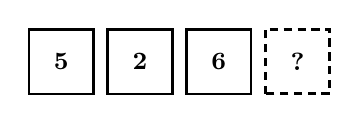
\begin{tikzpicture}[x=1cm, y=1cm, every node/.style={text=black}]
      \foreach \x/\d in {0/5, 1.0/2, 2.0/6} {
        \draw[black, line width=0.95pt, fill=white] (\x,0) rectangle (\x+0.82,0.82);
        \node[font=\small] at (\x+0.41,0.41) {\textbf{\d}};
      }
      \draw[black, line width=1.15pt, densely dashed, fill=white] (3.0,0) rectangle (3.82,0.82);
      \node[font=\small] at (3.41,0.41) {\textbf{?}};
    \end{tikzpicture}\\[4pt]
    \raggedright{\fontsize{8.3pt}{12.6pt}\selectfont
    ផលបូកដឹងស្រាប់៖ $5 + 2 + 6 + \square = 13 + \square$ ។\\[3pt]
    \textbf{(១) សោបើកពេល $\div 2$ និង $\div 3$៖} ខ្ទង់រាយគូ និង $13+\square$ ចែកដាច់នឹង $3 \Rightarrow \square \in \{\blank{1.6cm}\}$\\[3pt]
    \textbf{(២) សោបើកពេល $\div 5$ និង $\div 9$៖} រាយ $0$ ឬ $5$ និង $13+\square$ ដាច់នឹង $9 \Rightarrow \square = \blank{1.1cm}$}
  \end{tcolorbox}
\end{minipage}

\vspace{6pt}
% -------------------- ផ្នែក ង (E5 Diagnostic A--D + Exit Ticket 90s + Homework) --------------------
\secbox{ផ្នែក ង \enbf{(E5} វិនិច្ឆ័យ \enbf{A--D,} សំបុត្រចេញ និងកិច្ចការផ្ទះ\enbf{)}}{៤.៥ នាទី \en{+} កិច្ចការផ្ទះ $\le$២ នាទី}

\vspace{1pt}
\textbf{១. វិនិច្ឆ័យរហ័ស \en{A--D}៖} គូស \ding{51} លើ \textbf{ត្រូវ} ឬ \textbf{ខុស} រួចសរសេរលេខកូដយោង \cnum{1}--\cnum{4} ហើយលើកម្រាមដៃ (១=ត្រូវ, ២=ខុស) ព្រមគ្នា៖\\[3pt]
{\renewcommand{\arraystretch}{1.38}
\fontsize{8.4pt}{11.8pt}\selectfont
\begin{tabular}{|C{0.75cm}|L{9.30cm}|C{2.55cm}|L{4.75cm}|}
  \hline
  \cellcolor{panelgray}\textbf{ល.រ} & \cellcolor{panelgray}\textbf{អំណះអំណាងដែលត្រូវពិនិត្យ} & \cellcolor{panelgray}\textbf{វិនិច្ឆ័យ} & \cellcolor{panelgray}\textbf{កូដយោង \cnum{1}--\cnum{4} និងហេតុផល} \\ \hline
  \textbf{A} & «$19$ មានលេខខាងចុង $9$ ដូច្នេះវាចែកដាច់នឹង $9$ ។» & \chkbox\ ត្រូវ \ \chkbox\ ខុស & កូដ \blank{0.6cm}៖ \blank{3.1cm} \\ \hline
  \textbf{B} & «បើចំនួនមួយចែកដាច់នឹង $2$ ផង និង $5$ ផង ខ្ទង់រាយត្រូវជា $0$ ។» & \chkbox\ ត្រូវ \ \chkbox\ ខុស & កូដ \blank{0.6cm}៖ \blank{3.1cm} \\ \hline
  \textbf{C} & «$123$ ចែកដាច់នឹង $3$ ដូច្នេះវាច្បាស់ជាចែកដាច់នឹង $9$ ដែរ ។» & \chkbox\ ត្រូវ \ \chkbox\ ខុស & កូដ \blank{0.6cm}៖ \blank{3.1cm} \\ \hline
  \textbf{D} & «$2\,007$ ចែកដាច់នឹង $9$ ដូច្នេះវាច្បាស់ជាចែកដាច់នឹង $3$ ដែរ ។» & \chkbox\ ត្រូវ \ \chkbox\ ខុស & កូដ \blank{0.6cm}៖ \blank{3.1cm} \\ \hline
\end{tabular}}

\vspace{7pt}
\begin{minipage}[t]{9.25cm}
  \vspace{0pt}
  \begin{tcolorbox}[
    enhanced, sharp corners, colback=panelgray, colframe=black,
    boxrule=0.95pt, boxsep=2pt, top=5pt, bottom=6pt, left=5.5pt, right=5.5pt,
    equal height group=botboxes
  ]
    {\muol\fontsize{8.7pt}{12.2pt}\selectfont ២. សំបុត្រចេញ ៩០ វិនាទី \enbf{(Exit Ticket)}}\\[4pt]
    {\fontsize{8.6pt}{13.6pt}\selectfont
    រកលេខមួយខ្ទង់ដាក់ក្នុងប្រអប់ ដើម្បីឱ្យចំនួន $3\,\numbox\,25$ ចែកដាច់នឹង $9$ ៖\\[4pt]
    $\bullet$ ផលបូកខ្ទង់៖ $3 + \square + 2 + 5 = 10 + \square$\\
    $\bullet$ ដើម្បីឱ្យ $10 + \square$ ចែកដាច់នឹង $9$ (កូដ \cnum{4}) ត្រូវយក $\square = \blank{1.0cm}$\\
    $\bullet$ ផ្ទៀងផលបូកខ្ទង់ $= \blank{1.0cm}$ $\Rightarrow$ ចម្លើយ៖ $3\,\blank{0.6cm}\,25$ ។}
  \end{tcolorbox}
\end{minipage}\hfill%
\begin{minipage}[t]{9.25cm}
  \vspace{0pt}
  \begin{tcolorbox}[
    enhanced, sharp corners, colback=white, colframe=black,
    boxrule=0.95pt, boxsep=2pt, top=5pt, bottom=6pt, left=5.5pt, right=5.5pt,
    equal height group=botboxes
  ]
    {\muol\fontsize{8.7pt}{12.2pt}\selectfont ៣. កិច្ចការផ្ទះ \enbf{(}សៀវភៅគោល ទំ.២៤\enbf{)}}\\[4pt]
    {\fontsize{8.5pt}{13.3pt}\selectfont
    $\bullet$ \textbf{លំហាត់ទី១ (បញ្ជាក់ដោយមិនចែក)៖}\\
    \quad ក. $78+120$ ($\div 2$) \qquad ខ. $4\,140-720$ ($\div 3$)\\
    \quad គ. $165+270$ ($\div 5$) \qquad ឃ. $5\,130-342$ ($\div 9$)\\
    $\bullet$ \textbf{លំហាត់ទី២ ($734\square 0$)៖} បំពេញប្រអប់ឱ្យចែកដាច់៖ ក. នឹង $2$ ផង $5$ ផង; ខ. នឹង $3$ ផង $9$ ផង ។\\[3pt]
    \textit{ម៉ោងក្រោយ៖ អានមុនចំណុច ១.១គ ($4, 8$) និង ១.២ (ទំ.១៧--១៨)។}}
  \end{tcolorbox}
\end{minipage}

\end{document}
